\section{Data and methods}\label{sec:data-n-methods}

\subsection{Data}\label{subsec:data}

% Explain the apparatus and experimental technique

% Ran 5 experiments
% The blocks all my replicates in one side of the glasshouse
% Within the blocks they are all genetically different and in each block they have the same combinations
% 16 plants per plot
% Mutant population 

% 16 genotypes * 40 plots = 1 block each plant is genetically unique
% We need to link a specific genotype to a biomass
% Dsicovery system for genotypes - you create many random mutations and see if they exhibit this behaviour but because it is a random it needs to be done with manny genotypes

% This explains why the seeds are planted in transparent pots with the each seed planted just by the pot rim
Similarly,  \textit{Smith et al.}~\cite{smithSegmentationRootsSoil2020}have developed a pre-trained model for root segmentation from the side on transparent pot imagery. This technique has been developed for root segmentation where the seed is either planted in a transparent medium or planted in compost at the pot rim so shoots can be observed non-invasively.

% Explain manually annotating 280 images for training segmentation model using a semi-automated annotation pipeline

\subsection{Methods}\label{subsec:methods}

\begin{figure}
    \centering
    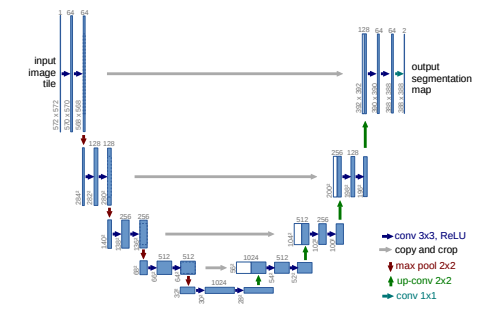
\includegraphics[width=0.5\linewidth]{assets//01_introduction/Screenshot 2024-05-22 at 16.06.04.png}
    \caption{Enter Caption}
    \label{fig:enter-label}
\end{figure}

U-Net was initially conceived for segmentation tasks in medical imaging but has seen widespread adoption in DL and Computer vision.
% TODO: basic background on U-Net with reference diagram (this should probably be moved to the methods section)
The U-Net model consists of two parts, which are mirror images of each other (see Figure~\ref{}).
The initial encoder part of the model takes the input image (or a smaller tile from the input image) and repeatedly applies convolution, followed by ReLU activation and Max pooling operations.
This reduces the spatial dimension of the image, producing a deep feature map.
This representation is then passed to the decoder part of the model with convolution layers that gradually increase the spatial dimension of the image, back to its original size.
U-Net also includes jump connections that connects the